% Homework Template
\documentclass[a4paper]{article}
\usepackage{ctex}
\usepackage{amsmath, amssymb, amsthm}
\usepackage{moreenum}
\usepackage{mathtools}
\usepackage{url}
\usepackage{bm}
\usepackage{enumitem}
\usepackage{graphicx}
\usepackage{subcaption}
\usepackage{booktabs} % toprule
\usepackage[mathcal]{eucal}
\usepackage[thehwcnt = 1]{iidef}

\thecourseinstitute{清华大学电子工程系}
\thecoursename{\textbf{媒体与认知} \space 课堂2}
\theterm{2021-2022学年春季学期}
\hwname{作业}
\begin{document}
\courseheader
\name{YOUR NAME}
\vspace{3mm}
\centerline{\textbf{\Large{理论部分}}}

\section{单选题(15分)}
\subsection{\underline{?}}

\subsection{\underline{?}}

\subsection{\underline{?}}

\subsection{\underline{?}}

\subsection{\underline{?}}

\section{计算题(15 分)}

\begin{figure}[h]
    \centering
    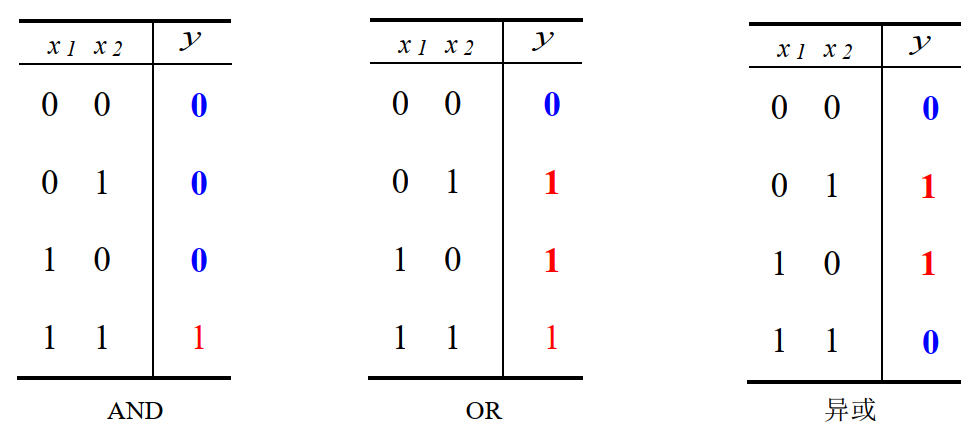
\includegraphics[width=12cm]{Fig1.png}
    \caption{AND,OR,异或三种逻辑运算}
    \label{fig:label_1}
\end{figure}

\subsection{基于如下单个人工神经元,设计实现两种逻辑门AND、OR运算。}
\begin{equation}
    z=w_1x_1 +w_2x_2 + b
\end{equation}
\begin{equation}
y=f(z)=\left\{
        \begin{array}{lr}
        1, z > 0 \\
        0, z \leq 0
        \end{array}
\right.
\end{equation}

\subsection{上述形式的单个神经元是否可以实现逻辑门异或运算?如果是,请给出具体设计;若否,请解释理由。}

\vspace{6mm}
\centerline{\textbf{\Large{编程部分}}}
\vspace{3mm}
% 请根据是否选择自选课题的情况选择“编程作业报告”或“自选课题开题报告”中的一项完成
\section{编程作业报告}
\section{自选课题开题报告}

\end{document}



%%% Local Variables:
%%% mode: late\rvx
%%% TeX-master: t
%%% End:
